
\documentclass[12pt, a4paper]{article}


%%%% Encodings

\usepackage[utf8]{inputenc} % encoding
\usepackage[english]{babel} % use special characters and also translates some elements within the document.

%%%% Misc

\usepackage{hyperref}       % Hyperlinks \url{url} or \href{url}{name}
\usepackage{parskip}        % \par starts on left (not idented)
\usepackage{tocbibind}      % Adds the bibliography to the table of contents (automatically)

% \usepackage[document]{ragged2e}  % Left-aligned (whole document)
% \begin{...} ... \end{...}   flushleft, flushright, center

%%%% Abstract

\usepackage{abstract}       % Abstract

% http://www.ctex.org/documents/packages/special/abstract.pdf
\renewcommand{\absnamepos}{flushleft} % \begin{abstract} \noindent ... \end{abstract}
\setlength{\absleftindent}{0pt}
\setlength{\absrightindent}{0pt}

%%%% Graphics

\usepackage{graphicx}
\graphicspath{{./figures/}} % directory to look up for graphics

% \begin{figure}[h]
%   \centering
%   \includegraphics[scale=0.5]{cat}  % [width=\textwidth, height=4cm],
%   \caption{Example of a cat}
%   \label{fig:cat}
% \end{figure}

%%%% Math

\usepackage{amsmath}        % Math
\usepackage{amssymb}        % New symbols http://milde.users.sourceforge.net/LUCR/Math/mathpackages/amssymb-symbols.pdf
\usepackage{bm}             % $\bm{D + C}$

\usepackage{amsthm} % Math, \newtheorem, \proof, etc
% \begin{theorem}\label{t:label}  ...  \end{theorem}
% \begin{proof} ... \end{proof}
\theoremstyle{plain} % default
\newtheorem{theorem}{Theorem}[section]
\newtheorem{corollary}{Corollary}[theorem]  % Numering depends on the current section (instead of global)
\newtheorem{lemma}[theorem]{Lemma} % Shares numeration with theorem.
\theoremstyle{definition}
\newtheorem{definition}{Definition}[section]
\theoremstyle{remark}
\newtheorem*{remark}{Remark}

% Defines a new environment to write your or claim - proof
\newenvironment{claim}[1]{\par\noindent\underline{Claim:}\space#1}{}
\newenvironment{claimproof}[1]{\par\noindent\underline{Proof:}\space#1}{\hfill $\blacksquare$}

%%%% Code/Pseudo-code

\usepackage{minted} % Code listing
% \mint{html}|<h2>Something <b>here</b></h2>|
% \inputminted{octave}{BitXorMatrix.m}

%\begin{listing}[H]
  %\begin{minted}[xleftmargin=20pt,linenos,bgcolor=codegray]{haskell}
  %\end{minted}
  %\caption{Example of a listing.}
  %\label{lst:example} % You can reference it by \ref{lst:example}
%\end{listing}

\newcommand{\code}[1]{\texttt{#1}} % Define \code{foo.hs} environment

\usepackage[vlined,ruled]{algorithm2e} % pseudo-code http://tug.ctan.org/macros/latex/contrib/algorithm2e/doc/algorithm2e.pdf

%%%% Colors

\usepackage{xcolor}         % Colours \definecolor, \color{codegray}
\definecolor{codegray}{rgb}{0.9, 0.9, 0.9}
% \color{codegray} ... ...
% \textcolor{red}{easily}

%%%% Math

%\makeglossaries % before entries

%\newglossaryentry{latex}{
    %name=latex,
    %description={Is a mark up language specially suited
    %for scientific documents}
%}

% Referene to a glossary \gls{latex}
% Print glossaries \printglossaries

\usepackage[acronym]{glossaries} %

% \acrshort{name}
% \acrfull{name}
% \newacronym{foo}{arcshort}{acrfull}

\usepackage{enumitem} % \begin{enumerate}[label=(\alph*)]



\usepackage{fancyhdr}
\pagestyle{fancy}
\fancyhf{}
\rhead{}
\lhead{}
\rfoot{Page \thepage}

\title{%
  \vspace{-10ex}
  Proposal: Stroke Prediction
}
\author{%
  Arnau Abella \\
  Antoni Casas \\
  \large{Universitat Polit\`ecnica de Catalunya}
}
\date{\today}

\begin{document}
\maketitle

\vspace{5ex}

\section{Introduction}
\label{sec:introduction}

Our problem is to \textbf{predict whether a patient is likely to get a stroke} based on
the input parameters such as age, diseases, smoking status and so.

We have chosen this problem because being able to predict stroke could prevent thousands of death per year since stroke is the second  cause of death in developed countries \cite{who}.

\section{The dataset}
\label{sec:dataset}

The dataset is from \href{https://www.kaggle.com/fedesoriano/stroke-prediction-dataset}{Kaggle}. The source is \textbf{confidential} since it contains personal data of patients of various hospitals.

The dataset is composed by:

\begin{itemize}
  \item 12 variables (7 numerical, 5 categorical)
  \item 5110 samples
  \item Only attribute \textit{bmi} has missing values.
  \item Some attributes have outliers e.g. \textit{age} and \textit{bmi}
  \item The dataset is imbalanced ($0.95$ --- $0.05$). We need to take this into consideration when doing the analysis.
\end{itemize}

The dataset has been previously studied (see \href{https://www.kaggle.com/fedesoriano/stroke-prediction-dataset/code}{previous work}).

\begin{table}[H]
\hskip-1.0cm\begin{tabular}{l|l|l}
Name                       & Type    & Categorical Range \\ \hline
Id                         & Numerical   &  \\
Gender                     & Categorical  & Male, Female, Other   \\
Age                        & Numerical & \\
Hypertension               & Binary   & 0 = no hypertension, 1 = hypertension   \\
Heart Disease              & Binary   & 0 = no hearth disease, 1 = heart disease  \\
Ever Married               & Binary  & No, Yes   \\
Work Type                  & Categorical  & Children, Gov. job, Never Worked, Private, Self employed   \\
Residence Type             & Categorical  & Rural, Urban   \\
Average Glucose Level      & Numerical &   \\
BMI (Body Mass Index)      & Numerical &   \\
Smoking Status             & Categorical  & Formerly smoked, never smoked, smokes, unknown   \\
Stroke                     & Binary   &   \\
\end{tabular}
\caption{Variables description}
\end{table}

\begin{figure}[H]
  \centering
  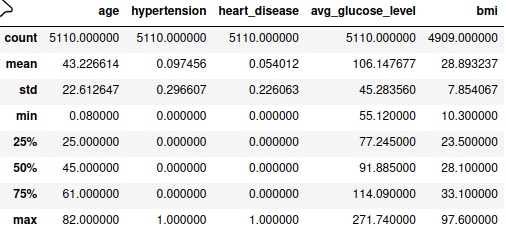
\includegraphics[scale=0.8]{describe}
  \caption{Numerical variables description}
  \label{fig:numerical}
\end{figure}

\bibliographystyle{unsrt}
\bibliography{refs}
\end{document}
